\section{Data samples.} \label{section:Data_samples}

	The detector was placed over a movable table which can be 
	displaced perpendicular to the beam line. Figure \ref{figure:zones} shows the definition of the coordinate system used to define the positions of the beam spot. 
	Furthermore, more run were along made the components to study the 
	uniformity of charge and efficiency.
	%it was necessary to take more runs to complete this analysis. %
	The beam momentum was set at 1 GeV/c for the general study of the
	components
	%; at 1.5 GeV/c for the pixel detector run;
	and another set at 1.5, 2 and 6 GeV/c for hitting at the center of the 
	plastic scintillator.
	%
	Unlike the use of the FEE in the ALICE environment, in T10 a 
	synchronization signal with the particles source 
	is not available, and the events occurs randomly, therefore we have to 
	define a reference for time; we mainly use T0-end detector to perform that 
	function. %
	Is worth to mention that the signal from the T0 detectors was changed from NIM to TTL level having a constant width and the charge was not measured. %
	The	width distribution of the T0-start have some events outside from a narrow distribution; meanwhile the T0-end distribution
	%(right from Figure \ref{figure:widthClean}) 
	shows a single narrow peak and to avoid that noise we select the events in a time window between 13 and 17 ns in T0-start. %
	
	\begin{figure}[ht!]
		\begin{center}
			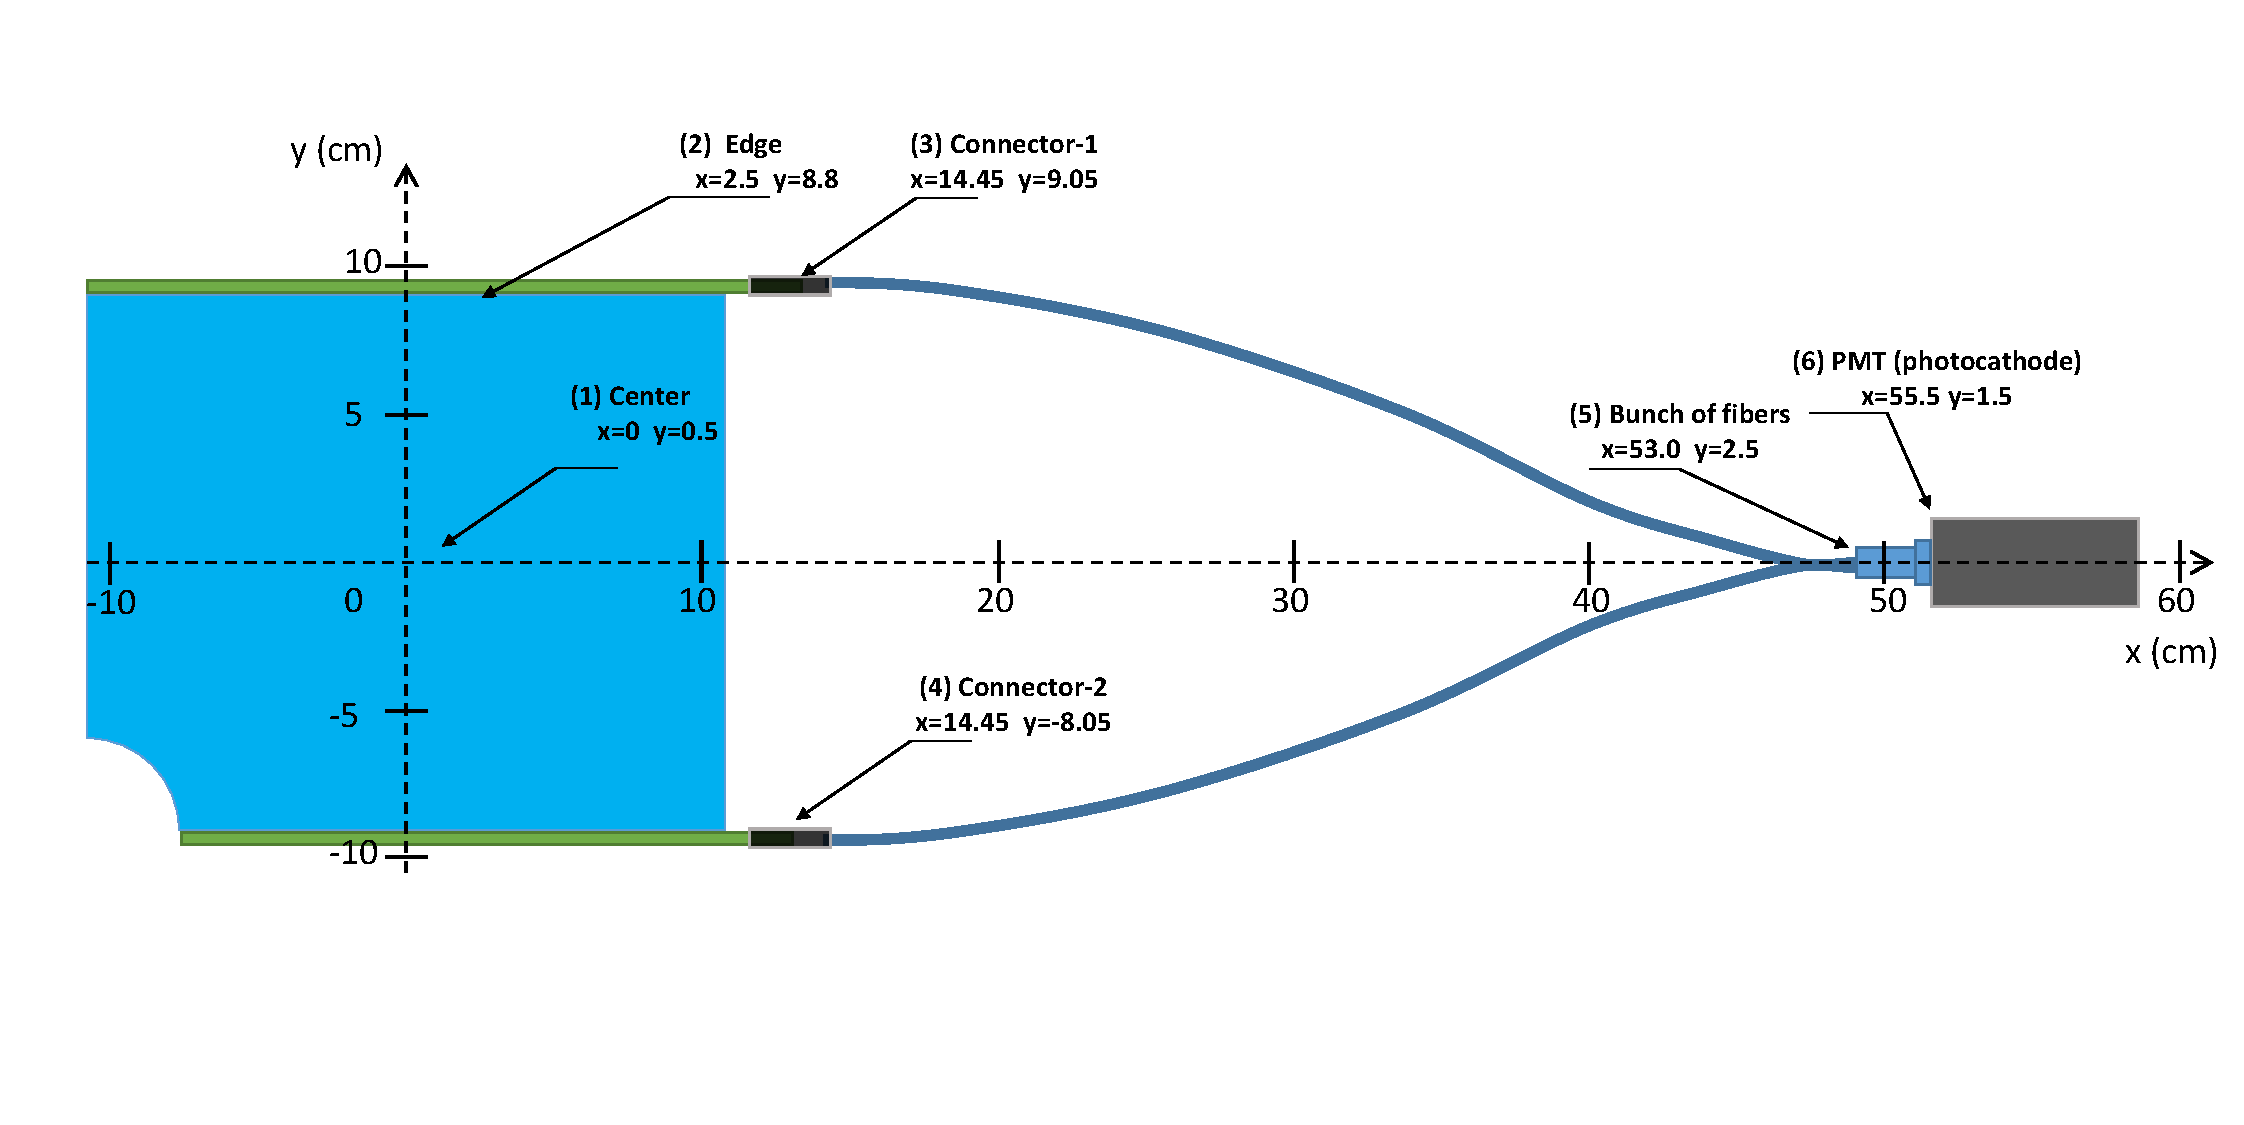
\includegraphics[scale=0.40]{./images/AD-2DNIM.pdf}
			\caption{
			Locations of the scintillator, the WLS bars, the fibers, and
				the PMT with respect to our coordinate system with origin at the center of the plastic scintillator.
			}
			\label{figure:zones}
		\end{center}
	\end{figure}

All those cleaning criteria were used along in furthers studies. Some other specific cleaning techniques
were applied depending on the particular characteristics of the analysis.
